\documentclass{mwart}
\usepackage[utf8]{inputenc}
\usepackage{indentfirst}
\usepackage{polski}
\usepackage{float}
\usepackage{hyperref}
\usepackage[caption = false]{subfig}
\usepackage[final]{graphicx}


\title{System rozpoznawania wybranych monet}

\author{
    Górka Bartosz\\
  \texttt{127228}
  \and
  Kruszyna Mateusz\\
  \texttt{127252}
}

\date{Poznań 01.12.2017}

\begin{document}

\maketitle

\newpage

\tableofcontents

\newpage

\section{Cel projektu}
Systemy automatycznego wnioskowania, rozpoznawania obrazów i wzorców stają się coraz bardziej popularne i wykorzystywane w codziennym życiu. Projekt miał na celu przygotowanie wstępnego zarysu programu komputerowego będącego w stanie rozpoznawać wybrane monety stosowane w Polsce.

Ograniczając projekt poprzez wyeliminowanie sztucznej inteligencji, system miał osiągnąć jak najlepszy wynik wykorzystując samą graficzną obróbkę plików źródłowych.

\section{Ograniczenia}
Przy przygotowaniu realizacji zabronione było wykorzystywanie w pełni gotowych rozwiązań ułatwiających wyszukiwanie monet i banknotów na obrazach. Zabronione było wykorzystanie \textit{klasyfikatora Haara}, który rozwiązałby większość problemów. Dodatkowo wszelkiego rodzaju \textit{OCR} również był zakazany.

Jako ułatwienie przyjęto ograniczenie analizowanych monet i banknotów do unikatowych kolorystycznie tj. \textit{0,05 PLN, 1 PLN, 2 PLN, 5 PLN, 10 PLN, 50 PLN, 100 PLN}.

\section{Historia pracy nad algorytmem}
Przygotowanie algorytmu do wykrywania obiektów na obrazie nie jest rzeczą trywialną. Wiele czynników może negatywnie oddziaływać na proces analizy. Są to między innymi różnice w naświetleniu obiektu, refleksy, czy też sama jakość zdjęcia.
Prace rozpoczęto od wykrywania monet na obrazie, aby następnie poddać analizie i określić z jaką monetą mamy do czynienia.

Na sam początek zaproponowano, aby odróżniac monety po kolorach, co w pierwotnej wersji okazało się bardzo słabe (a dokładniej implementacja tego pomysłu zawiodła). Przeglądając dalej dostępne funkcje w dokumentacji oraz prace naukowe o przetwarzaniu obrazów, chcieliśmy skupić się na różnych fakturach monet. Korzystając z różnej struktury monety (co szczególnie widoczne jest po zastosowaniu algorytmu detekcji krawędzi - \textit{Sobel}) pragnęliśmy zastosować wiedzę o  \textit{momentach Hu} oraz \textit{filtru Gabora} do analizy tekstury.
Niestety obydwa wyżej wymienione sposoby wymagają jasno określonego wzorca, który nie jest możliwy do osiągnięcia w naszych zastosowaniach. W przypadku monet, nawet sztucznie wygenerowane przekształcenia, nie były wystarczająco wierne w stosunku do oryginałów. Problem spowodowany był precyzją w wycinaniu obiektu z obrazu, gdyż różnica kilku pikseli znacząco wpływała na wynik porównania.

Po analizie niepowodzenia z implementacją tak rozbudowanego porównania, postanowiliśmy zmienić sam sposób podejścia do wykrytego obiektu. Zamiast porównywać fakturę, powróciliśmy do sprawdzenia kolorów, ale z innym nastawieniem (na różnice między kolorami, a nie ich wartości w wybranej przestrzeni barw). Pozwoliło to wyprowadzenie zależności dotyczących klasy obiektu.

\section{Analiza algorytmu}
\subsection{Wyszukiwanie monet}

Wyszukiwanie monet odbywa się dzięki użyciu funkcji \textit{findContours} z biblioteki OpenCV. Wykorzystanie tej funkcji pozwala na wykrywanie kształtów, w tym okręgów, które są dla nas najbardziej istotne, poprzez funkcję \textit{minEnclosingCircle}.
Niestety sama funkcja zwraca bardzo wiele obiektów, które trzeba poddać analizie w celu eliminacji błędów. Sytuację bez tego kroku można zaobserwować poniżej.

\begin{center}
    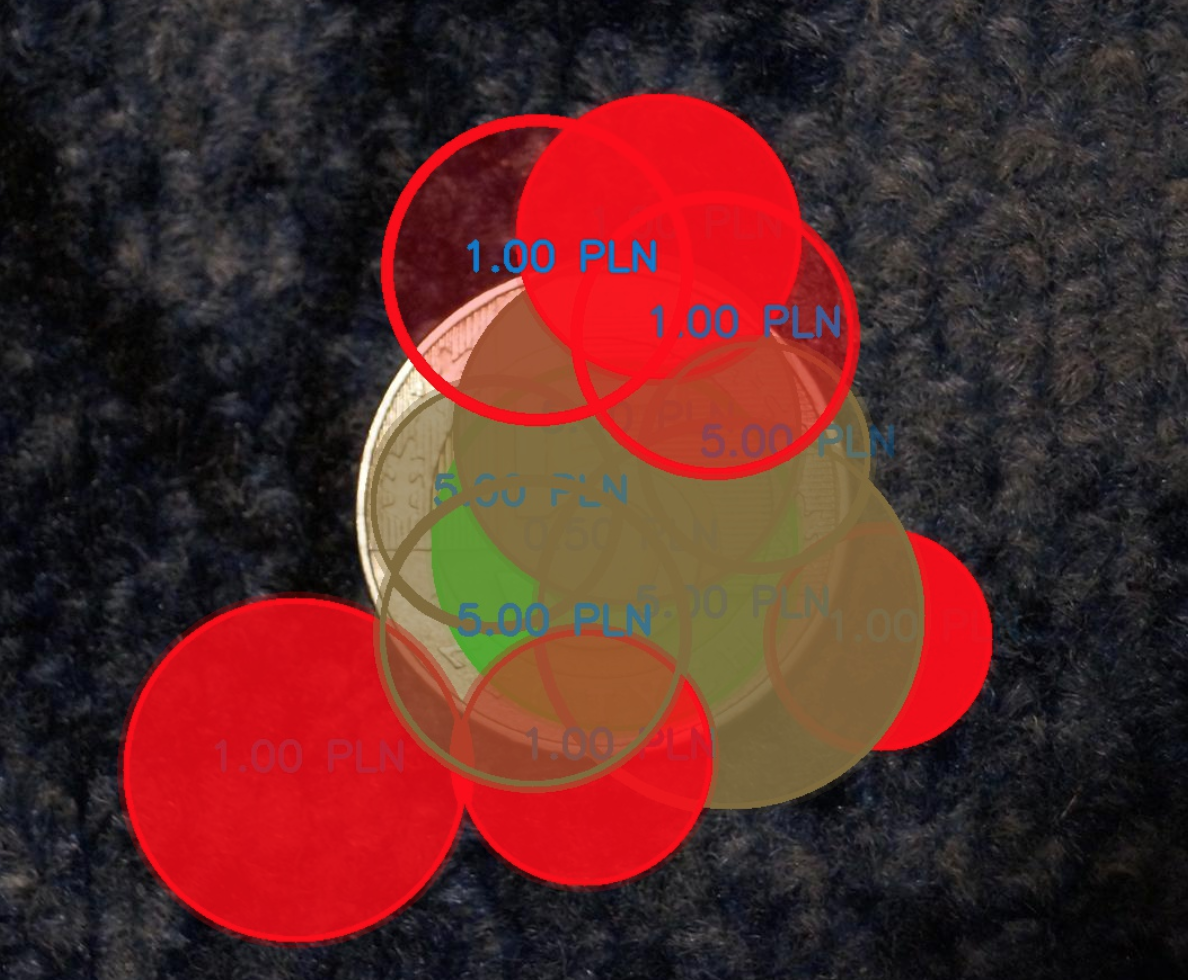
\includegraphics[width=\textwidth]{Objects.png}
\end{center}

Aby tego uniknąć, w algorytmie zastosowano różne opcje wykrywania obrazu i jego parametrów. W zależności od średniej wartości kanału V w przestrzeni barw \textit{HSV} algorytm wybiera odpowiedni preprocesing obrazu.

Dla ciemnych obrazów $V_avg < 100$ wprowadza się dużą korekcję gamma \textit{15} oraz skalowanie intesywności obrazu w zależności od percentyli.
W tym miejscu otrzymujemy obraz binarny (czarne tło oraz białe obiekty).
Następnie ścieżka wykrywania kół rozchodzi się na dwie ścieżki. Jedna przetwarza obraz za pomocą operacji morfologicznych, a druga używa funkcji \textit{Canny} oraz operacji morfologicznych. Wynik tych dwóch ścieżek jest łączony (operator \&) i przekazywany do funkcji \textit{findContours}.

Dla jasnych obrazów $V_avg >= 100$ wprowadza się przeciwną korekcję gammy \textit{0.7}. Dalej algorytm korzysta z funkcji \textit{adaptiveThreshold} z parametrem \textit{cv2.ADAPTIVE\_THRESH\_GAUSSIAN\_C} oraz operacji morfologicznych. Wynik przekazywany jest do funkcji \textit{findContours}.

Wykrywanie kół odbywa się poprzez funkcję \textit{minEnclosingCircle} i sprawdzenie czy pole wykrytej figury nie jest zbyt małe, albo zbyt duże, oraz czy jest w przybliżeniu równe polu koła $\Pi * r^2$. Pozwala to na pominięcie kształtów, które zostały po wstępnym przetworzeniu obrazu, tak jak na obrazkach poniżej.

\begin{center}
    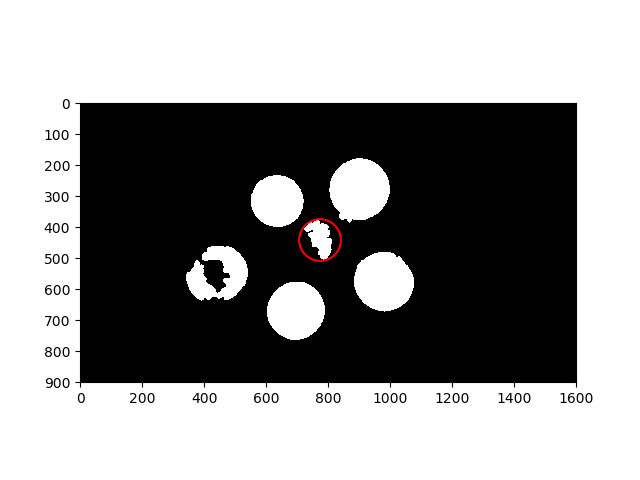
\includegraphics[width=\textwidth]{Area.png}
    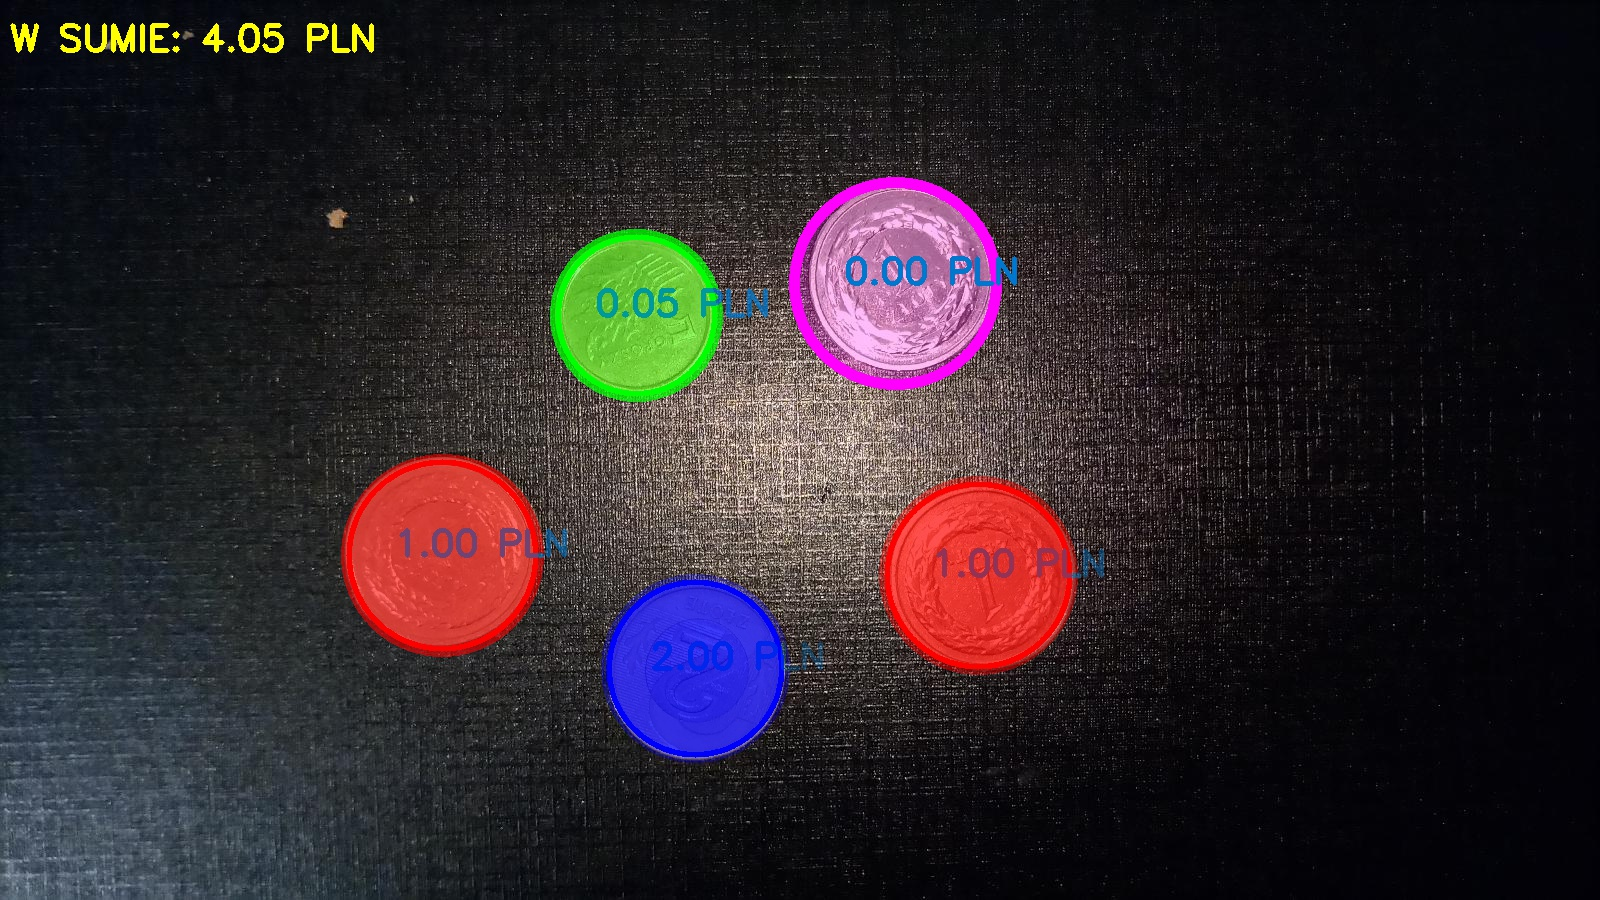
\includegraphics[width=\textwidth]{bb_000.jpg}
\end{center}

\subsection{Wyszukiwanie banknotów}
Poszukiwanie konturów, które mogą być potencjalnymi prostokątami zawierającymi banknoty, wymaga sprawdzenia wielu warunków.

Obraz podawany jest detekcji krawędzi \textit{Canny}, z wartościami progowania \textit{0, 50} oraz wielkością maski \textit{5x5} pikseli. Rezultat działania poddany jest dylatacji, dzięki której wyszczególniamy nasze krawędzi.

Banknot \textit{10 PLN} w kolejnych krokach algorytmu.
\begin{center}
    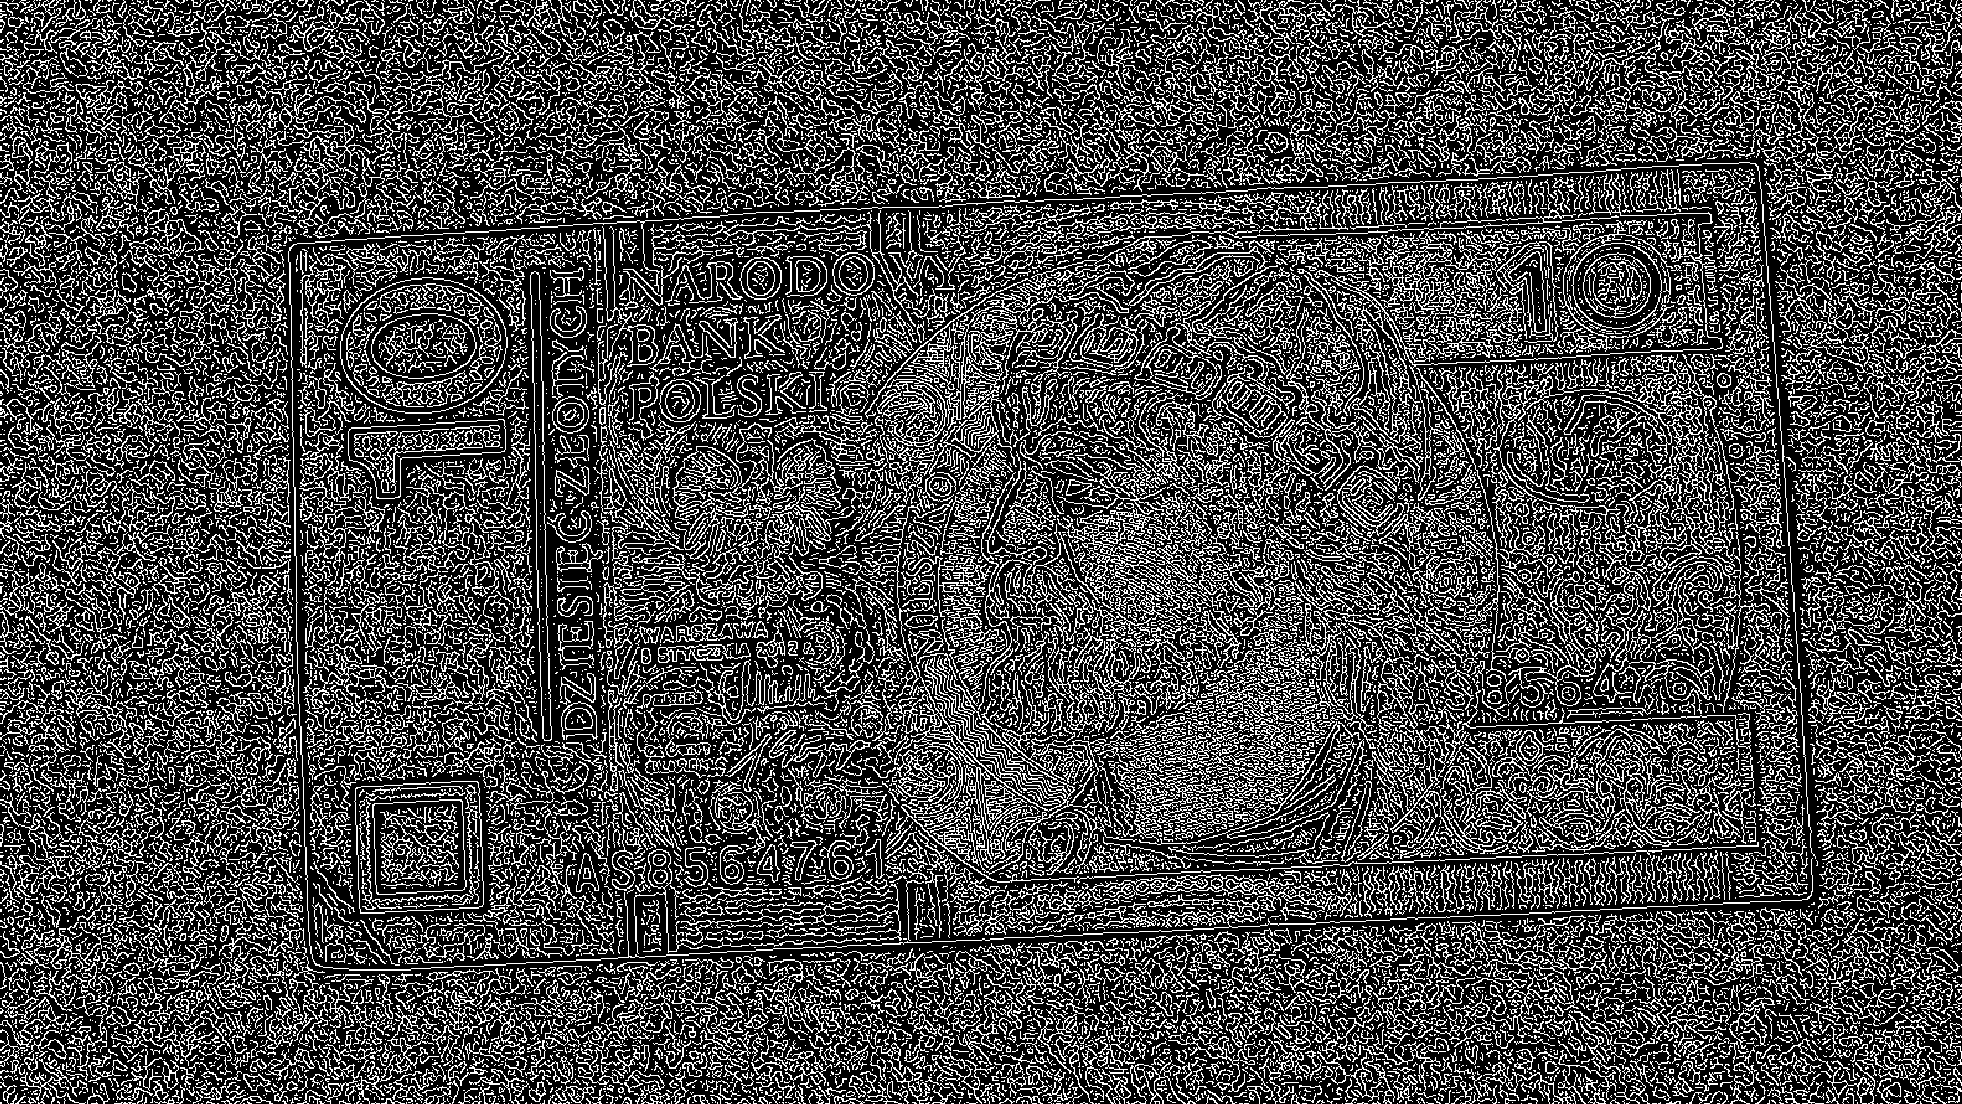
\includegraphics[width=\textwidth]{Gray_10_before.png}
\end{center}

\begin{center}
    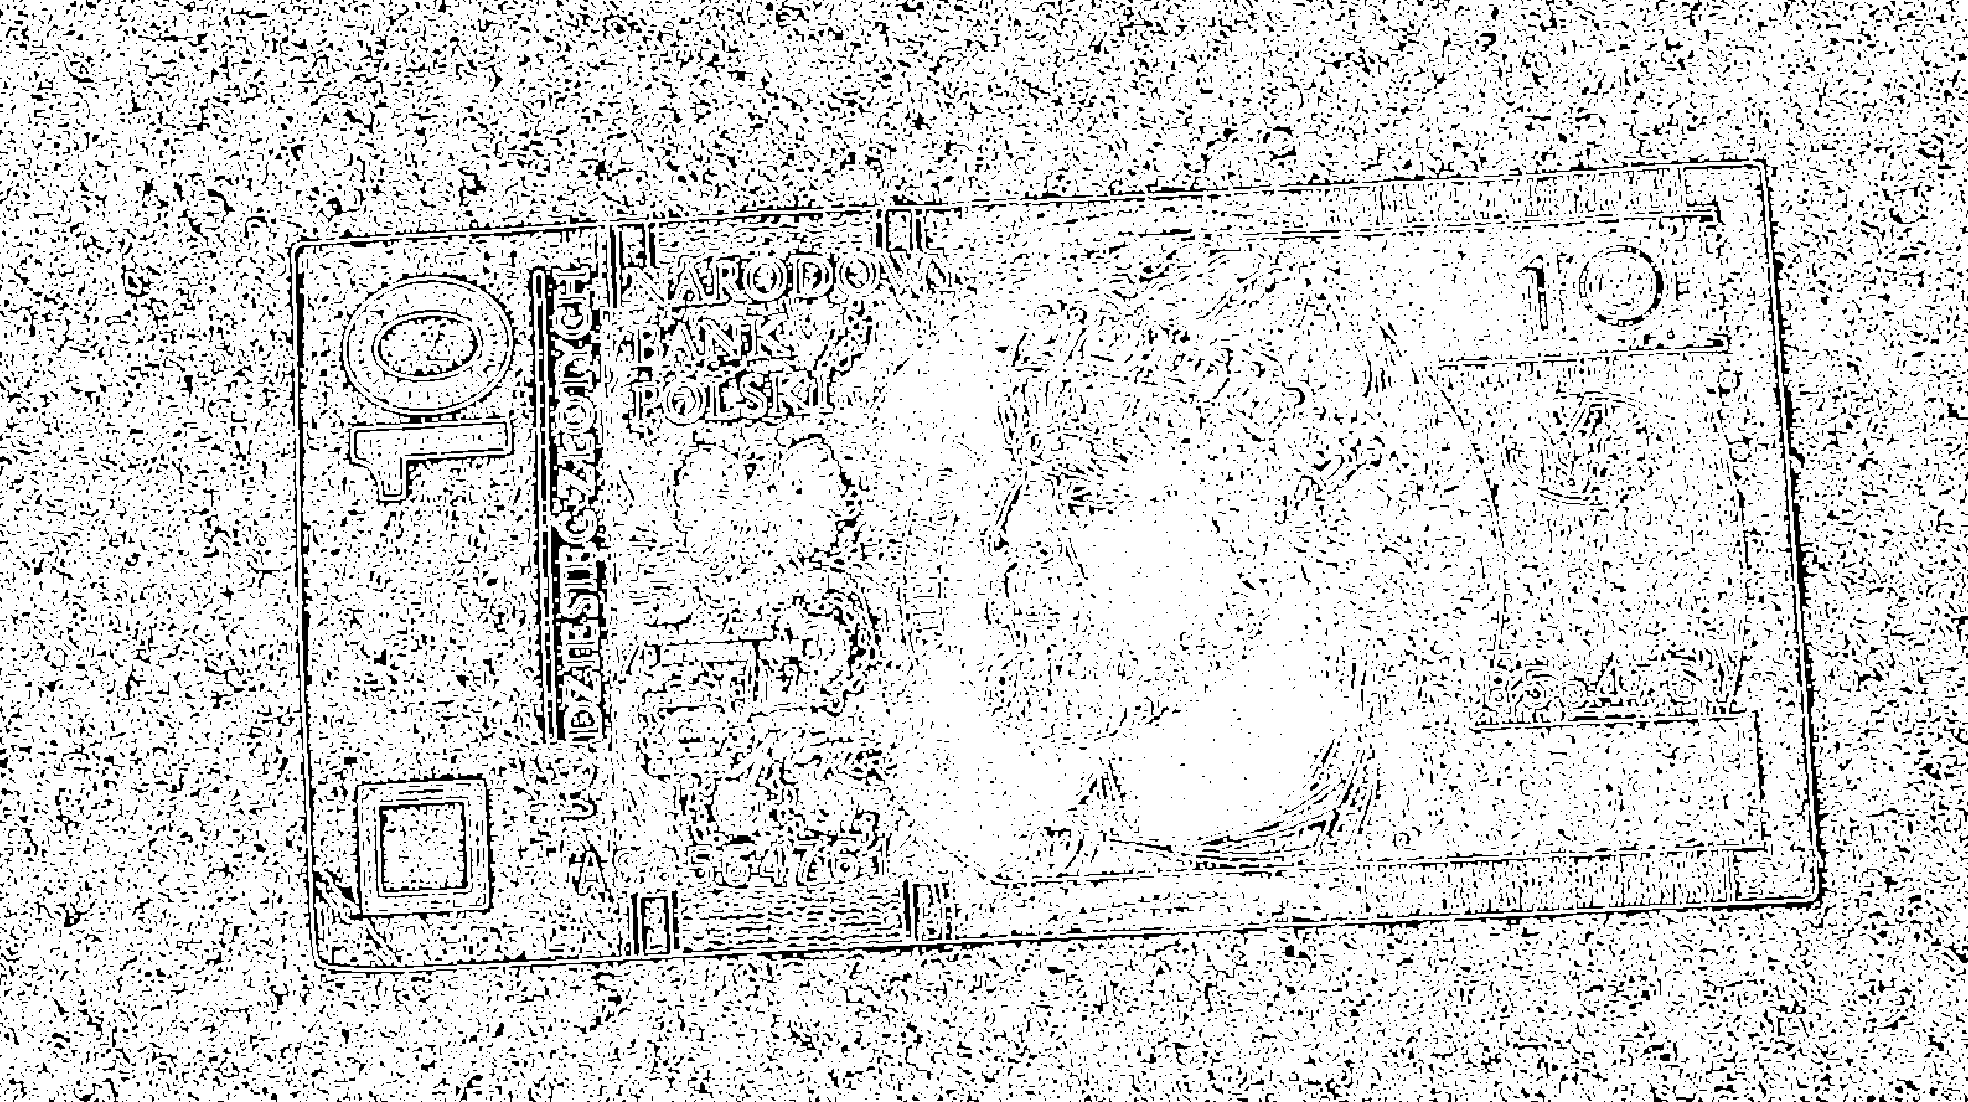
\includegraphics[width=\textwidth]{Gray_10_after.png}
\end{center}

Jak widać, ostatnie zdjęcie ułatwia wyszukanie konturów banknotu, gdyż stały się one szczególnie widoczne. Analizując poniższe zdjęcie, możemy zauważyć, że bez dodatkowych zabezpieczeń w postaci sprawdzania kątów między krawędziami oraz dolnego limitu pola powierzchni, znaleziono by zbyt dużo obiektów. Po wprowadzeniu wymienionych warunków, otrzymujemy pożądany wynik.

\begin{center}
    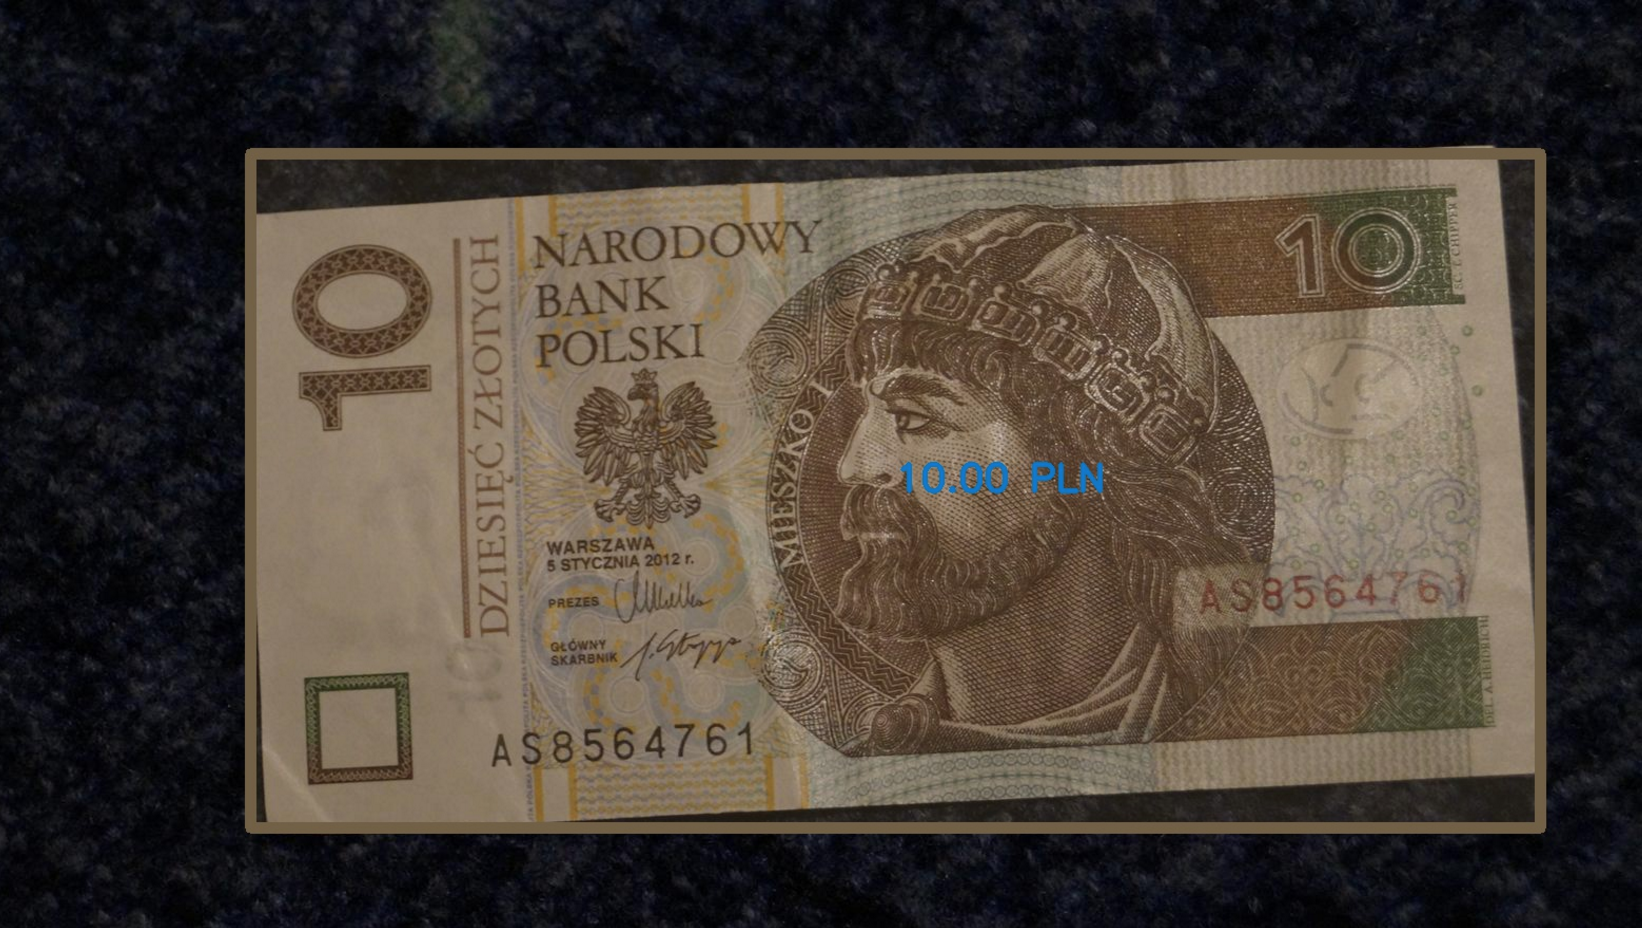
\includegraphics[width=\textwidth]{Single_10_PLN.png}
\end{center}

\subsection{Sposób rozpoznawania monet}

Wykorzystana została właściwość badanych obiektów, jakim u nas jest różnica w barwach wnętrza monety oraz jej obrzeża.

Dzięki takiemu postępowaniu możemy wydedukować, z którą z czterech kombinacji mamy do czynienia. Sukcesy w rozpoznawaniu monet zostają niestety ograniczone przez wykorzystaną funkcję Wymaga ona podania minimalnego oraz maksymalnego promienia, które bez wcześniejszej ingerencji ze strony operatora mogą wyeliminować z obliczeń zdjęcia zawierające zbyt małe, bądź też zbyt duże obiekty.

\begin{center}
    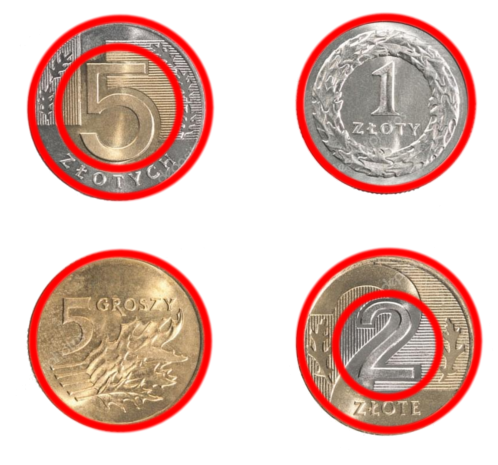
\includegraphics[width=\textwidth]{money.png}
\end{center}

Na początku wycinane jest wnętrze obiektu i dodawane analizie kolorów. Nastepnie ta sama czynność dotyczy przygotowanego pierścienia.

Każdy z pikseli innych od czarnego \textit{(R: 0, G: 0, B: 0)}, który zostały dodane przez nas jako tło maski, jest analizowany. Obliczamy sumę wartości bezwględnych różnic pomiędzy poszczególnymi częściami koloru tj. \textit{r - g, r - b, g - b}. Suma ta jest dodawana do tablicy wartości cząstkowych, która na samym końcu zostaje uśredniona dzięki zastosowaniu \textit{numpy.average}.

W drodze eksperytmu z przygotowanymi zdjęciami, wybrano następujące zakresy:

$$
decyzja = \left\{\begin{array}{ll}
\textrm{zignorowanie} & \textrm{gdy średnia $<$ 20}\\
\textrm{srebro} & \textrm{gdy średnia $<$ 120}\\
\textrm{złoto} & \textrm{gdy średnia $\geq$ 120 }
\end{array} \right.
$$

Kluczowym etapem jest poprawne przygotowanie elementu do analizy. Niestety również taka implementacja jest wyjątkowo wrażliwa na prześwietlone obiekty, które człowiek rozpozna bez wielkiego problemu, a dla systemów rozpoznawania nie jest to takie proste.

\subsection{Sposób rozpoznawania banknotów}

Próby rozpoznania banknotów rozpoczęto podobnie jak w przypadku monet. Początkowe podejście z liczeniem średniej dla całego banknotu zostało szybko zarzucone, aby liczyć średnią tylko dla wybranego wycinka. Wykorzystano korzystną właściwość występowania na banknocie władcy Polski w różnym kolorze.

\begin{center}
    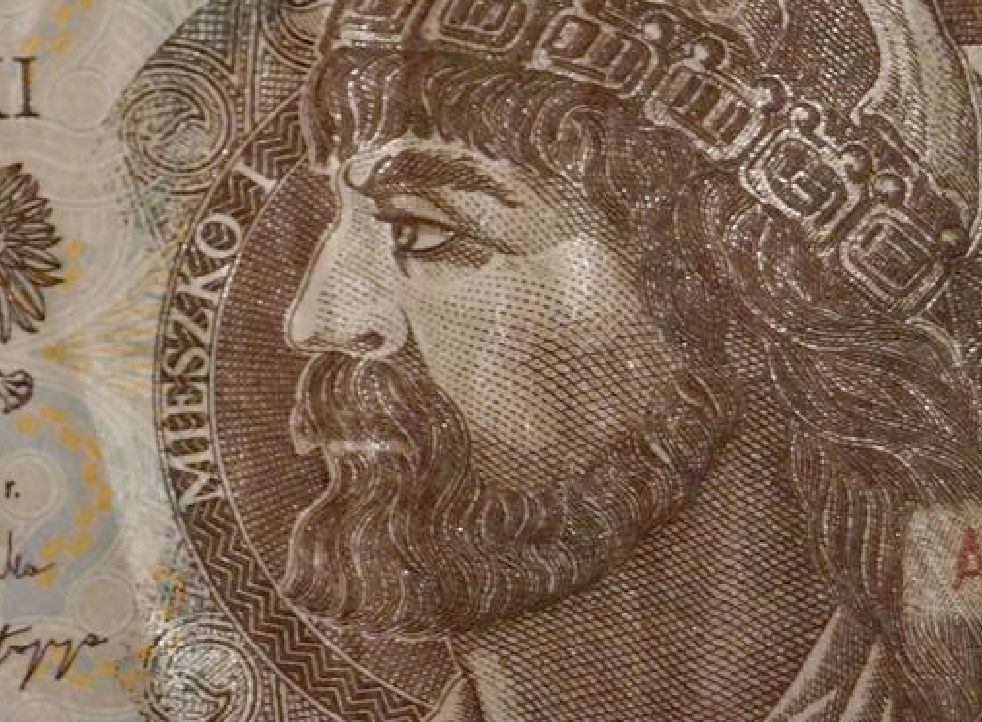
\includegraphics[width=\textwidth]{10_PLN_part.png}
\end{center}

W drodze eksperytmu z przygotowanymi zdjęciami, wybrano następujące zakresy dla wnioskowania odnośnie banknotu:

$$
decyzja = \left\{\begin{array}{ll}
\textrm{10 PLN} & \textrm{gdy średnia $>$ 80}\\
\textrm{50 PLN} & \textrm{gdy średnia $>$ 40}\\
\textrm{100 PLN} & \textrm{gdy średnia $\leq$ 40 }
\end{array} \right.
$$

\section{Wnioski}
Analizując zachowanie się algorytmu dla wszystkich przygotowanych zdjęć, można zauważyć jego niedoskonałości wymagające poprawy. Pierwszą rzeczą jest sposób wykrywania potencjalnych monet czy banknotów (ogólnie lepsze wykrywanie krawędzi tego czego chcemy).
Następnie można by poprawić detekcję monet, ale jest to trudne ponieważ kolory zdjęcia są przeróżne (nie mówiąc już o na przykład kolorowym światle z lapmki).

Prowadząc eksperymenty z ustawieniami programu, przygotowanymi zdjęciami testowymi czy zastosowanymi rozwiązaniami, można zauważyć potrzebę użycia sztucznej inteligencji w projekcie.
Rozpoznawanie obiektów dla człowieka wydaje się rzeczą naturalną, niestety dla komputera nie jest to trywialny problem. Próba podejścia do zagadnienia bazując wyłącznie na kolorach nie spełnia naszych oczekiwań, gdyż wiemy jak łatwo spreparować zdjęcia dla których algorytm odniesie sromotną porażkę.

\section{Analizowane przypadki}

\subsection{Pomyślne rozpoznanie}
\begin{figure}[ht!]
     \begin{center}
        \subfigure[1]{
            \label{fig:first}
            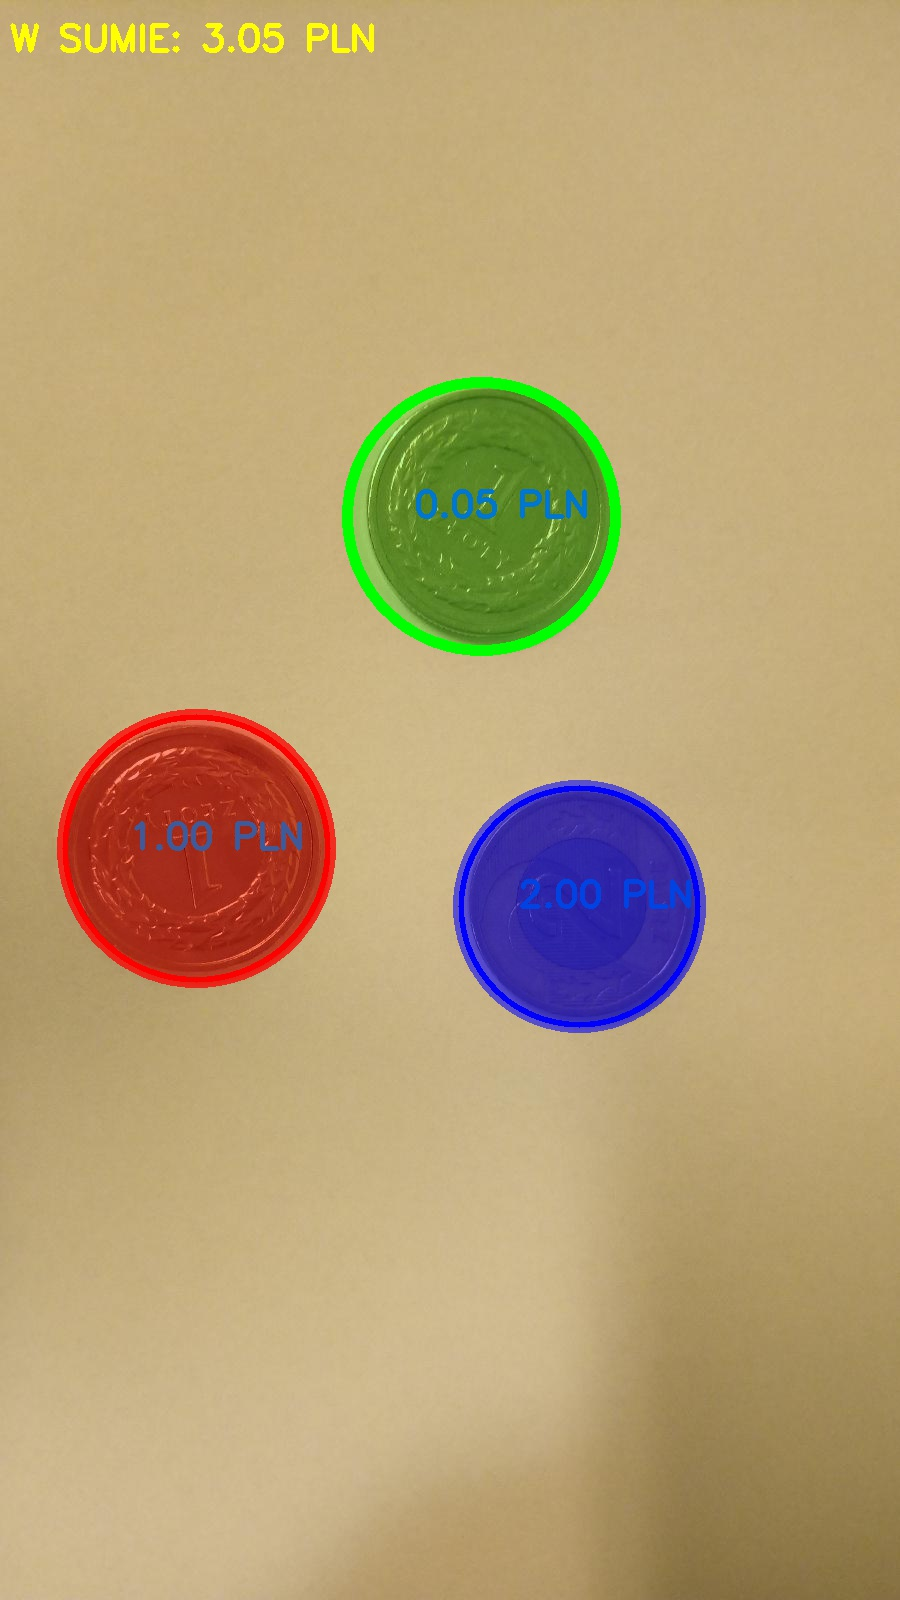
\includegraphics[width=0.4\textwidth]{good_001.jpg}
        }
        \subfigure[2]{
           \label{fig:second}
           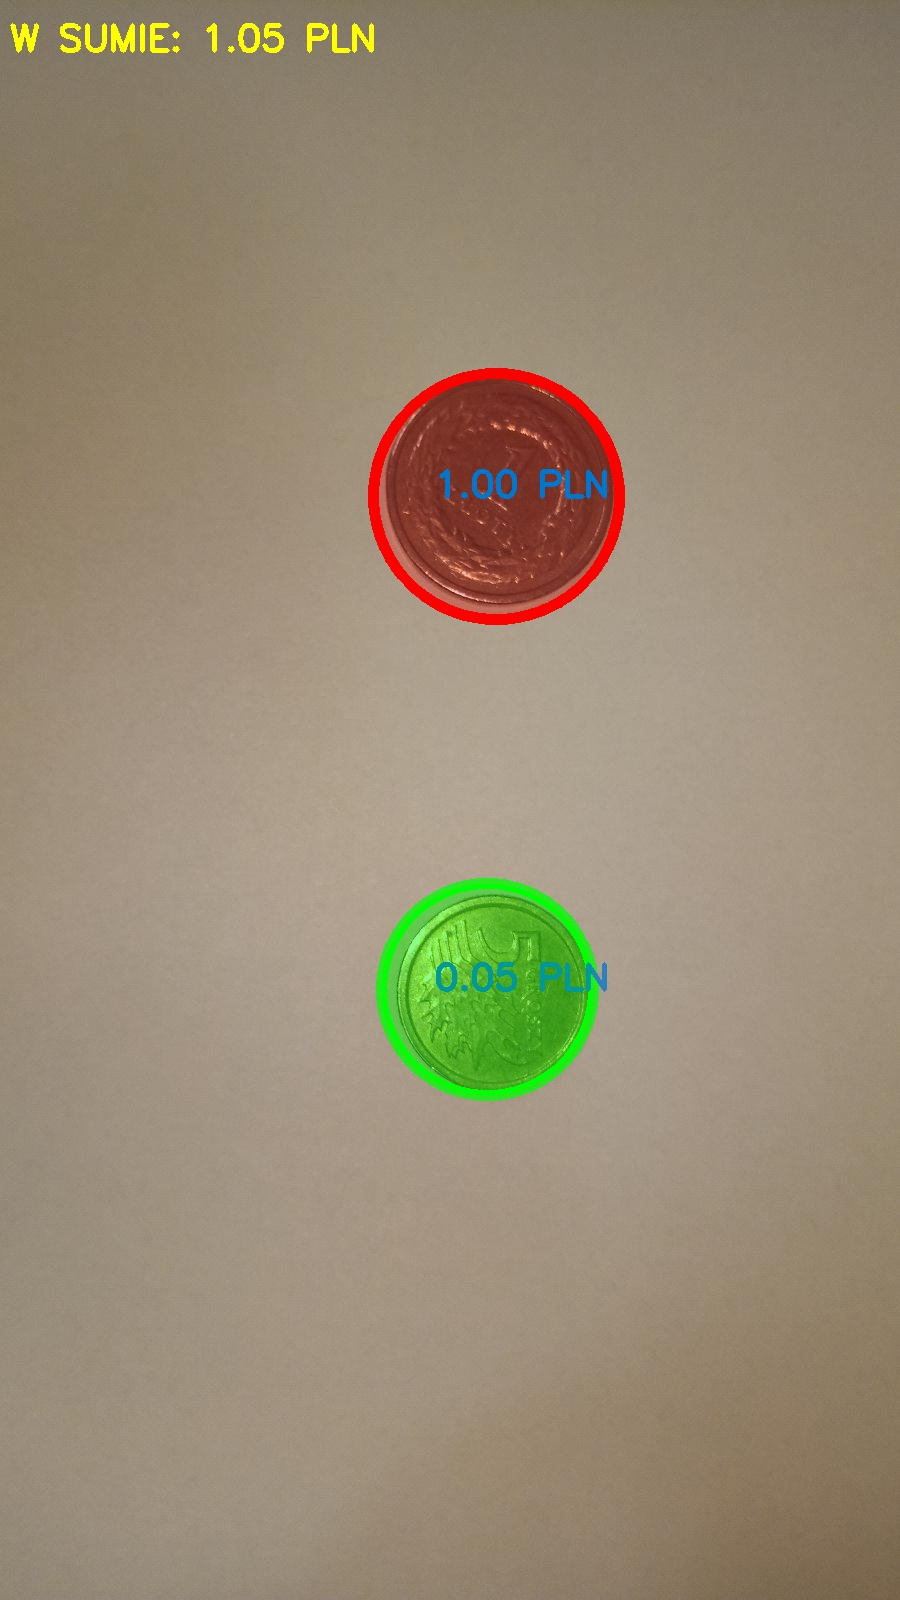
\includegraphics[width=0.4\textwidth]{good_002.jpg}
        }\\
        \subfigure[3]{
            \label{fig:third}
            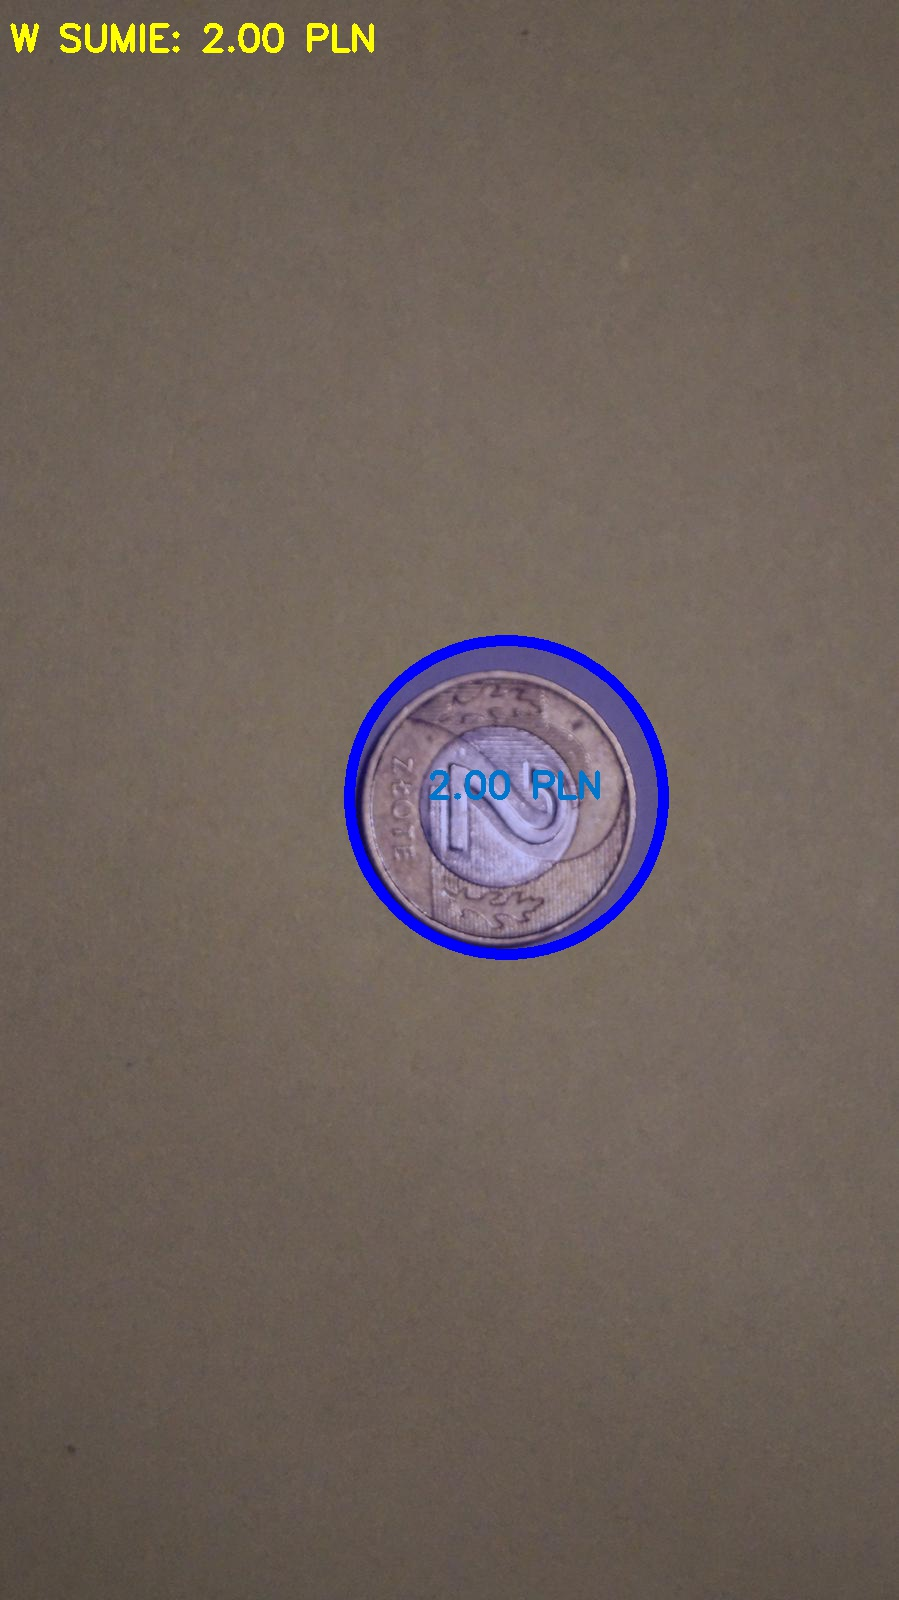
\includegraphics[width=0.4\textwidth]{good_004.jpg}
        }
        \subfigure[4]{
            \label{fig:fourth}
            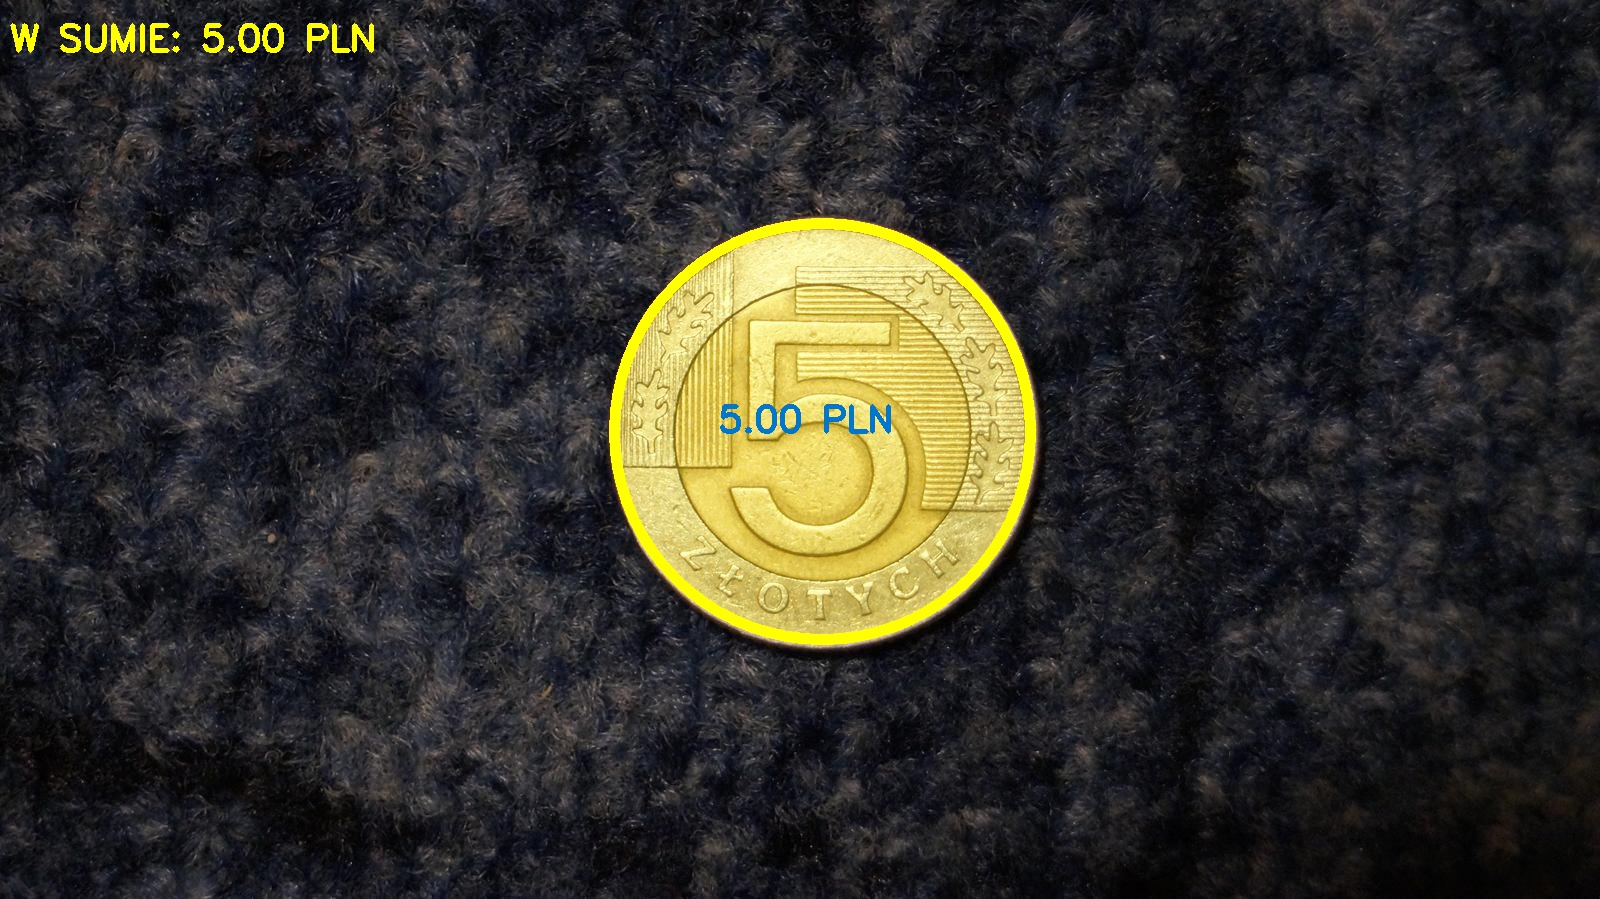
\includegraphics[width=0.4\textwidth]{good_005.jpg}
        }
    \end{center}
    \caption{Pomyślnie rozpoznane obrazki (1)}
   \label{fig:subfigures}
\end{figure}


\begin{figure}[ht!]
     \begin{center}
        \subfigure[1]{
            \label{fig:first}
            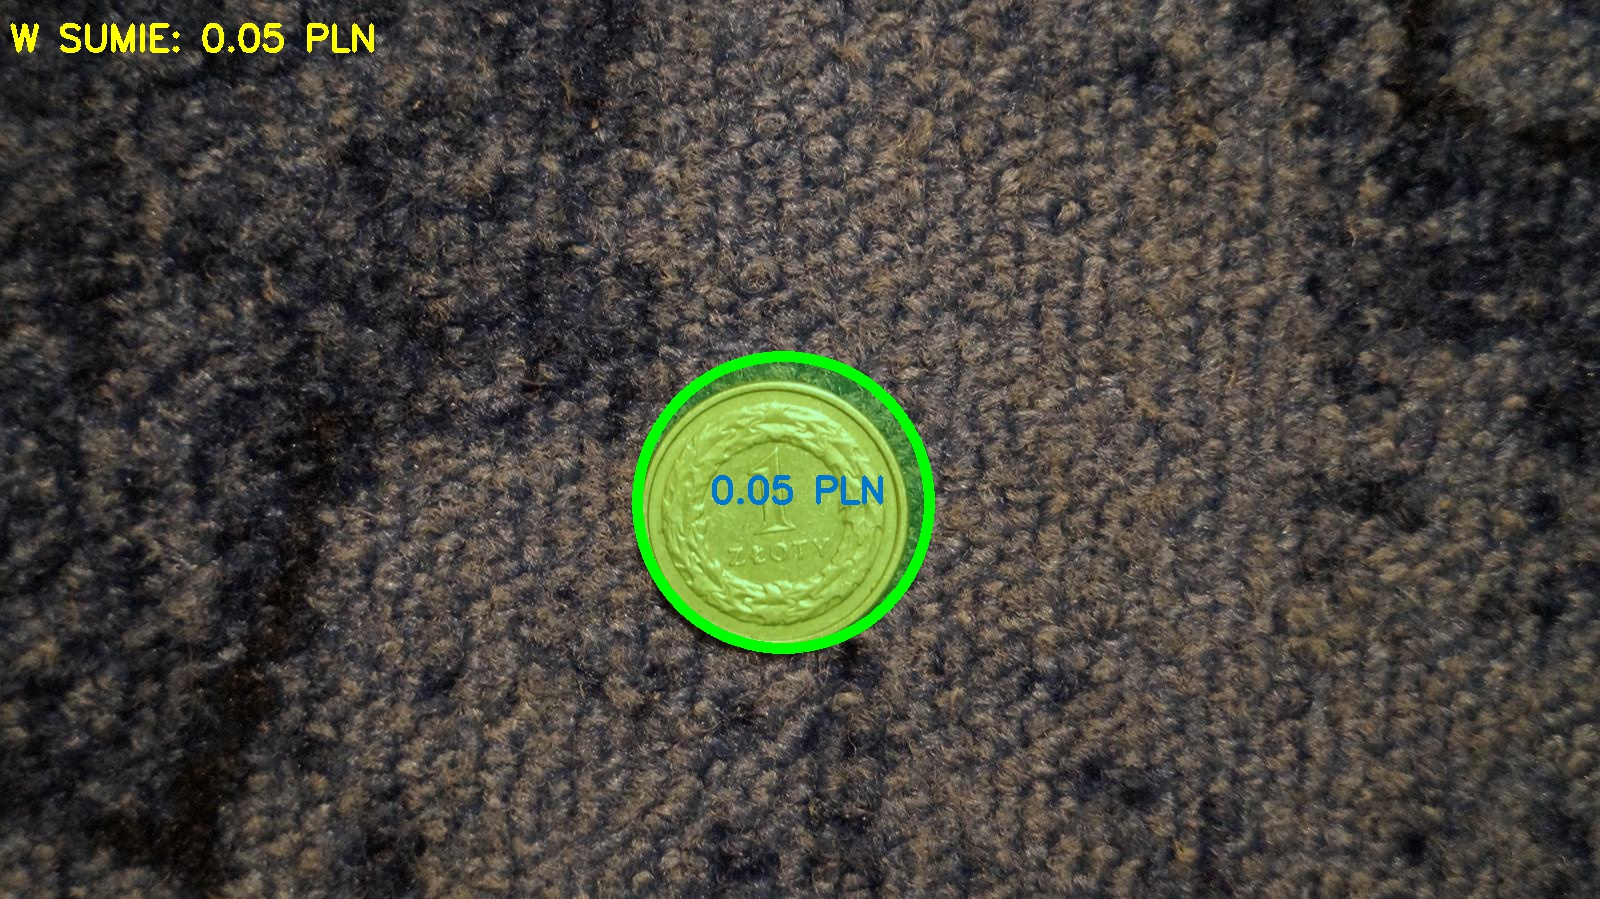
\includegraphics[width=0.4\textwidth]{good_006.jpg}
        }
        \subfigure[2]{
           \label{fig:second}
           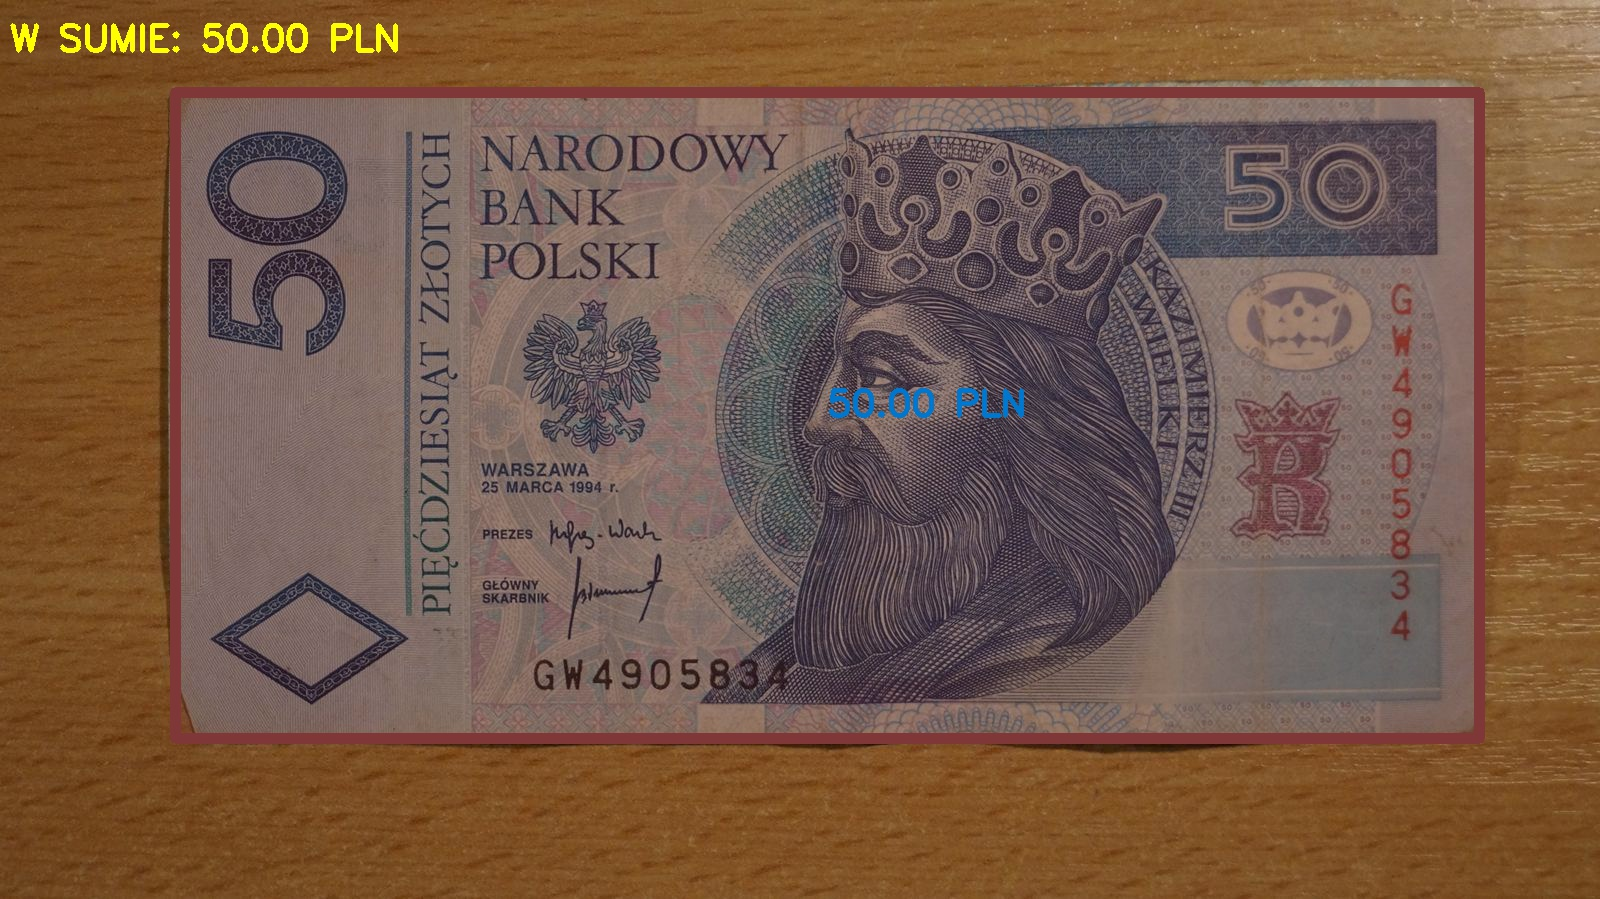
\includegraphics[width=0.4\textwidth]{good_007.jpg}
        }\\
        \subfigure[3]{
            \label{fig:third}
            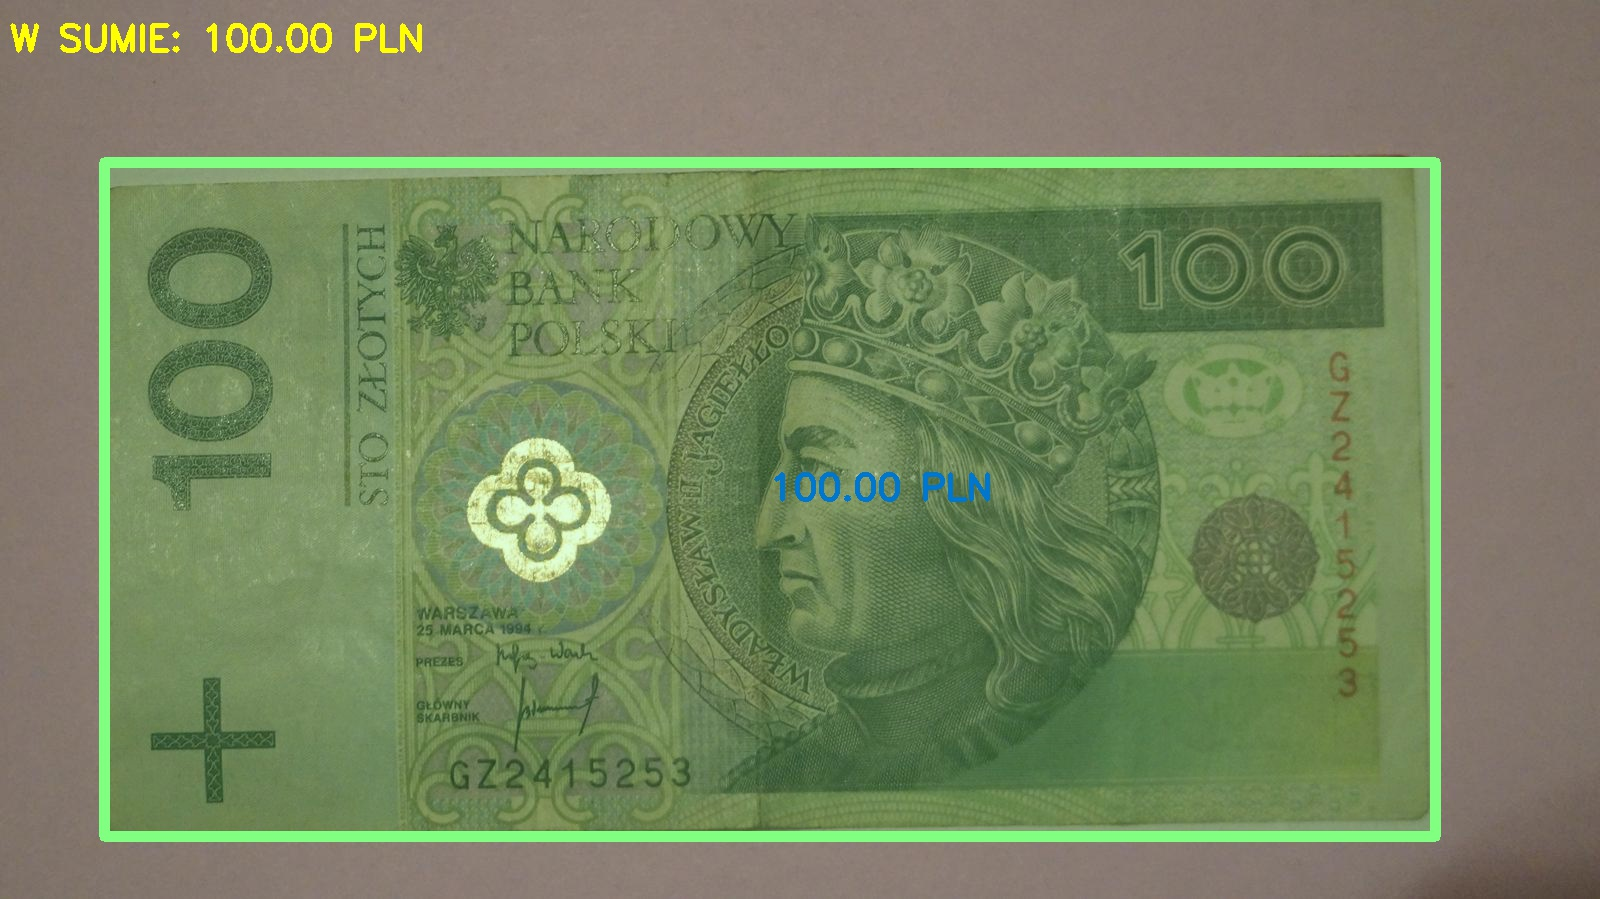
\includegraphics[width=0.4\textwidth]{good_008.jpg}
        }
        \subfigure[4]{
            \label{fig:fourth}
            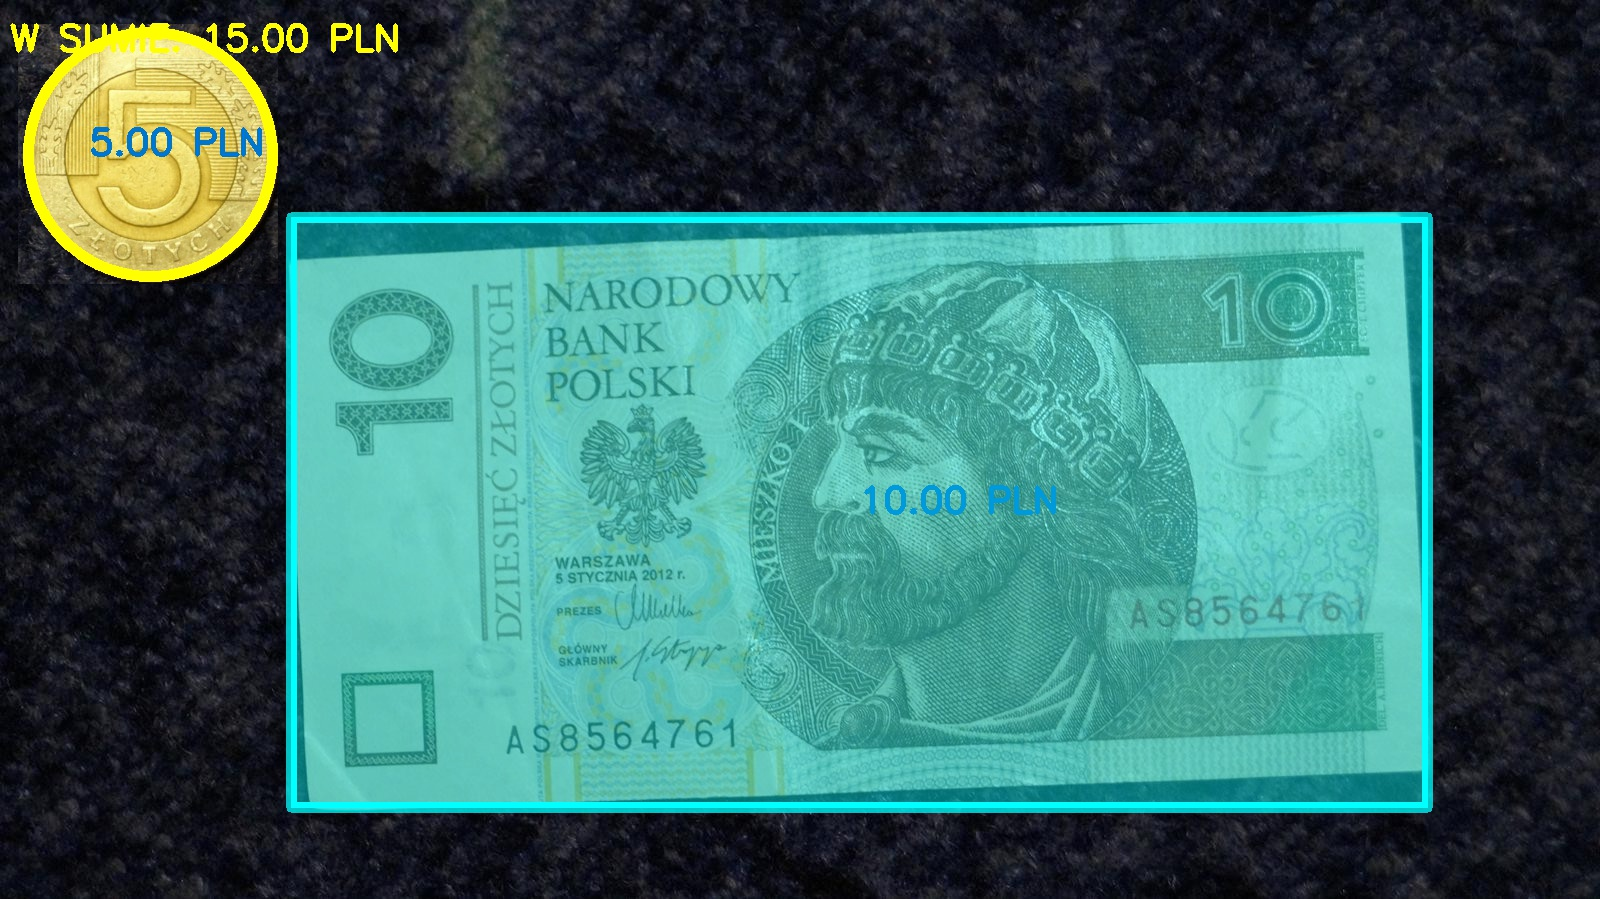
\includegraphics[width=0.4\textwidth]{good_009.jpg}
        }
    \end{center}
    \caption{Pomyślnie rozpoznane obrazki (2)}
   \label{fig:subfigures}
\end{figure}


\subsection{Niepomyślne rozpoznania}
\begin{figure}[ht!]
     \begin{center}
        \subfigure[1]{
            \label{fig:first}
            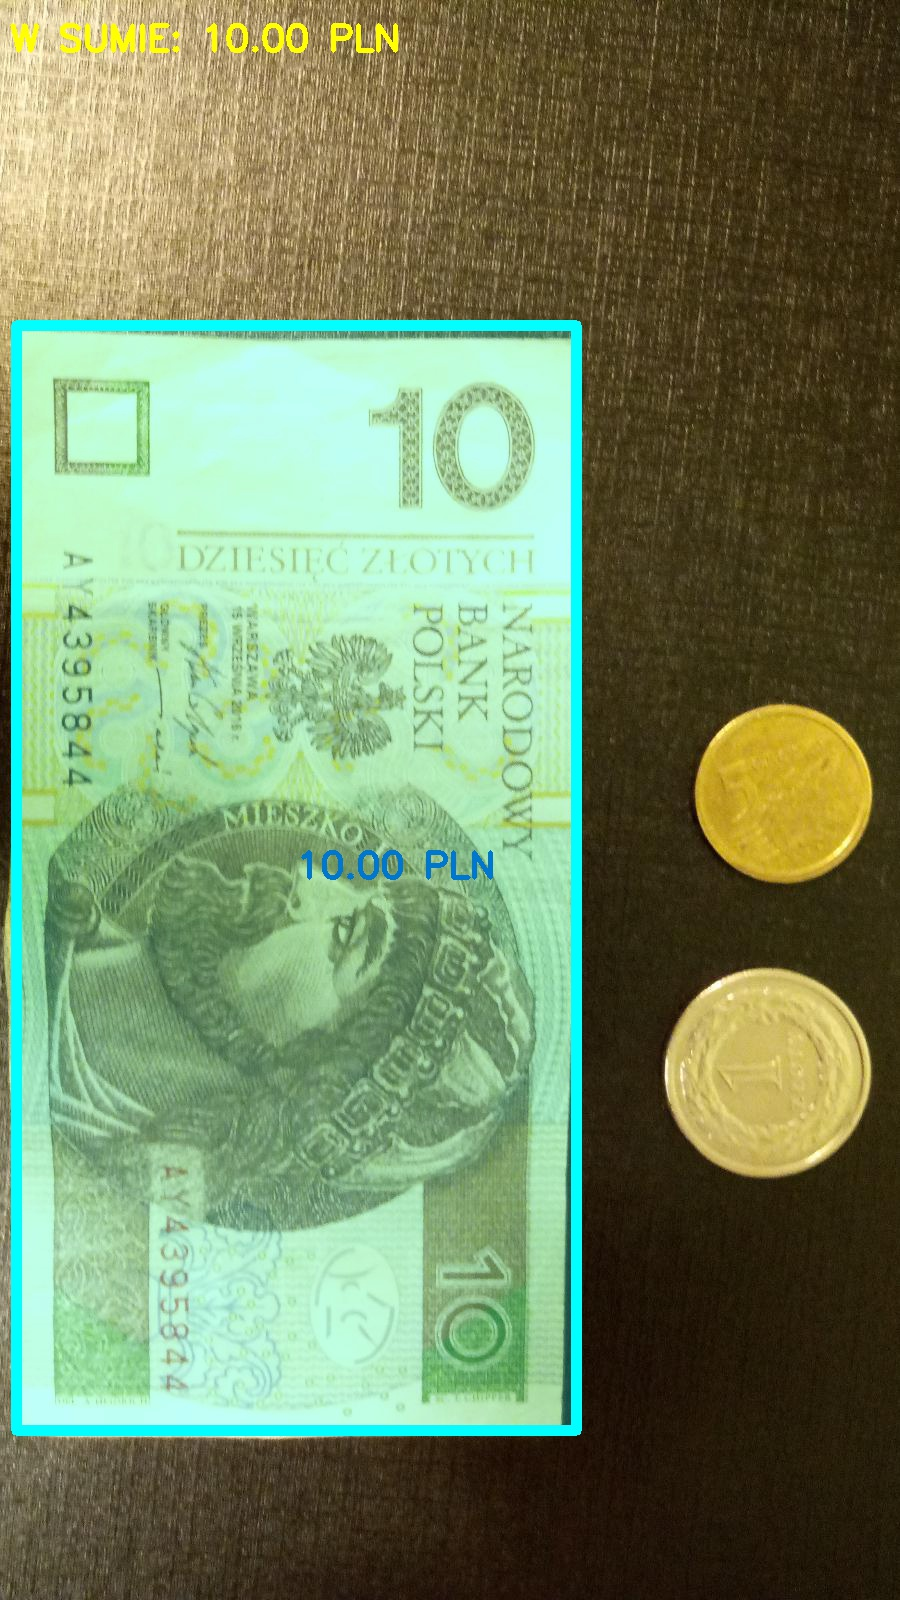
\includegraphics[width=0.4\textwidth]{bad_001.jpg}
        }
        \subfigure[2]{
           \label{fig:second}
           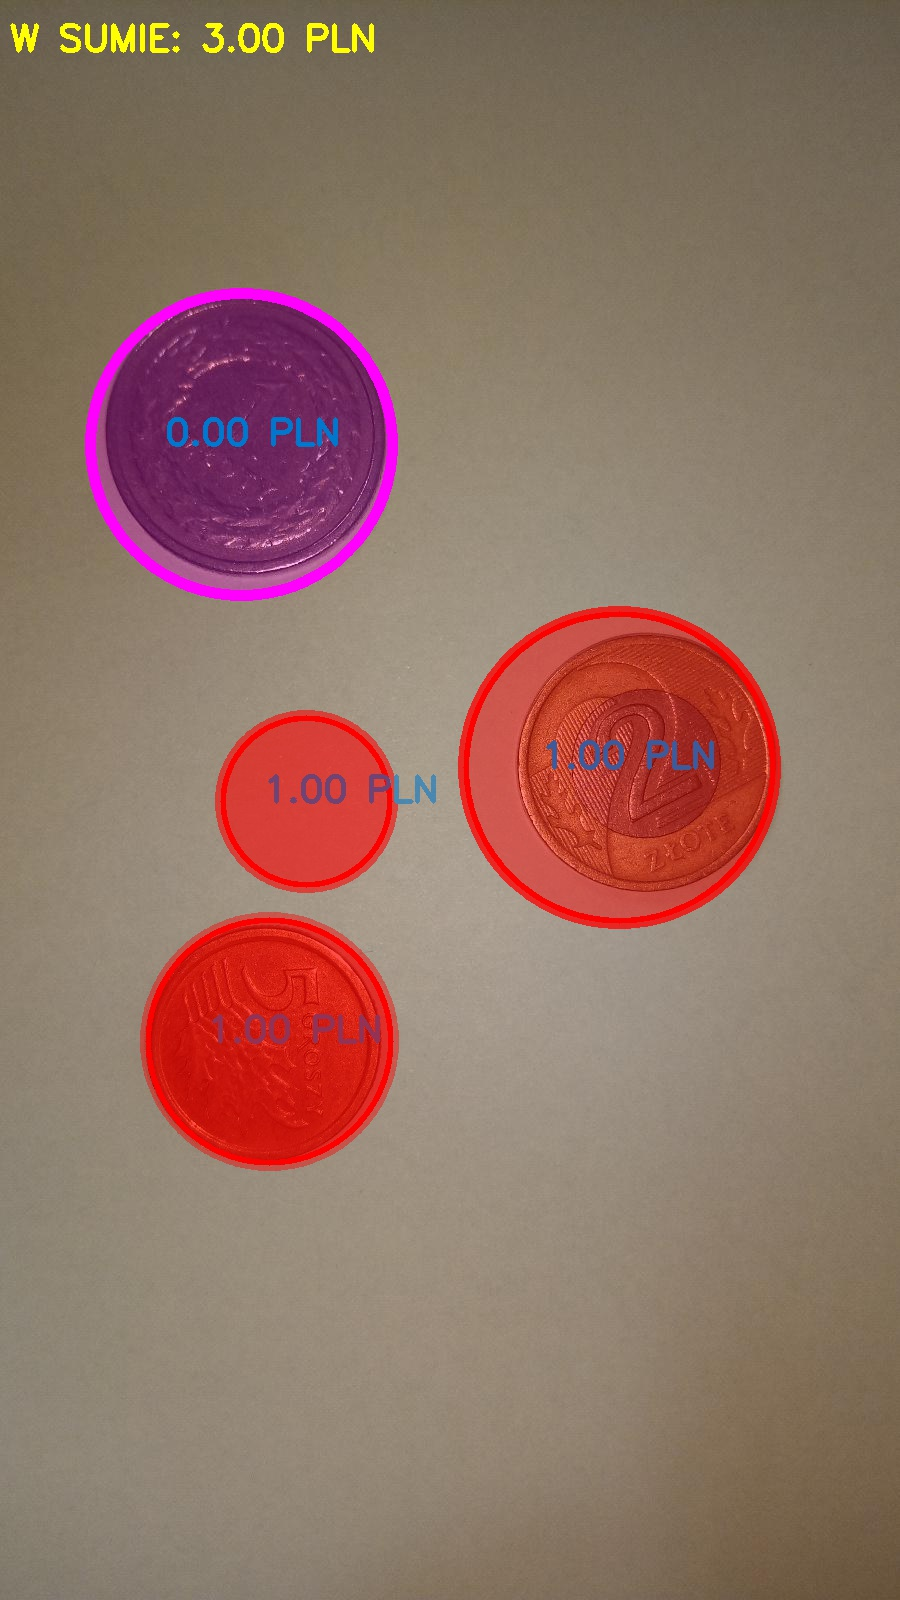
\includegraphics[width=0.4\textwidth]{bad_002.jpg}
        }\\
        \subfigure[3]{
            \label{fig:third}
            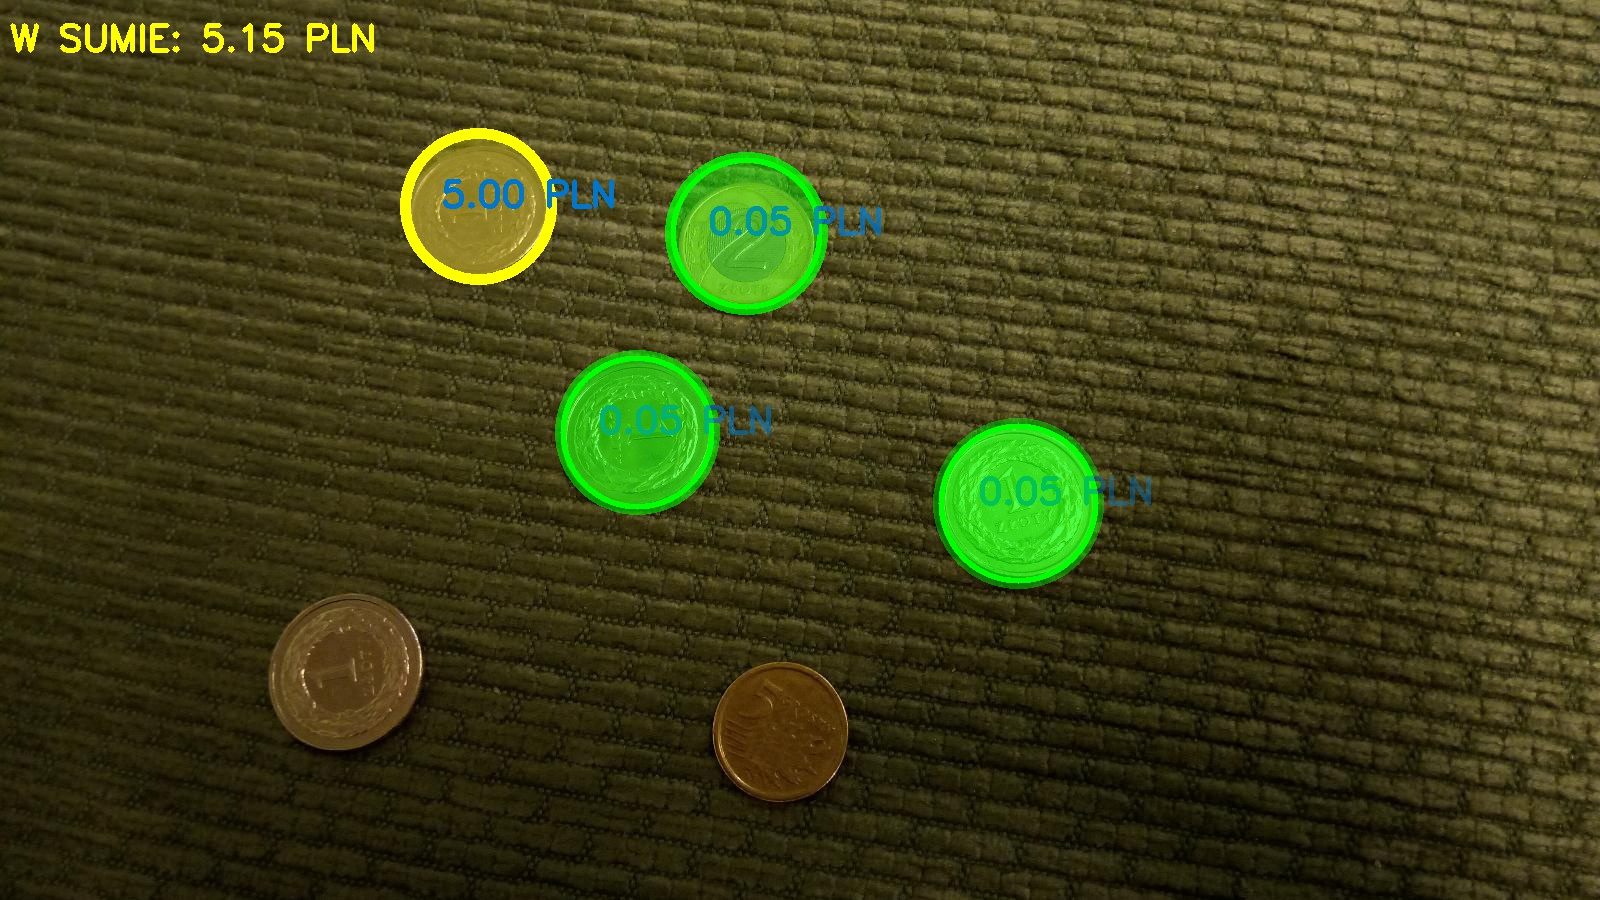
\includegraphics[width=0.4\textwidth]{bad_003.jpg}
        }
        \subfigure[4]{
            \label{fig:fourth}
            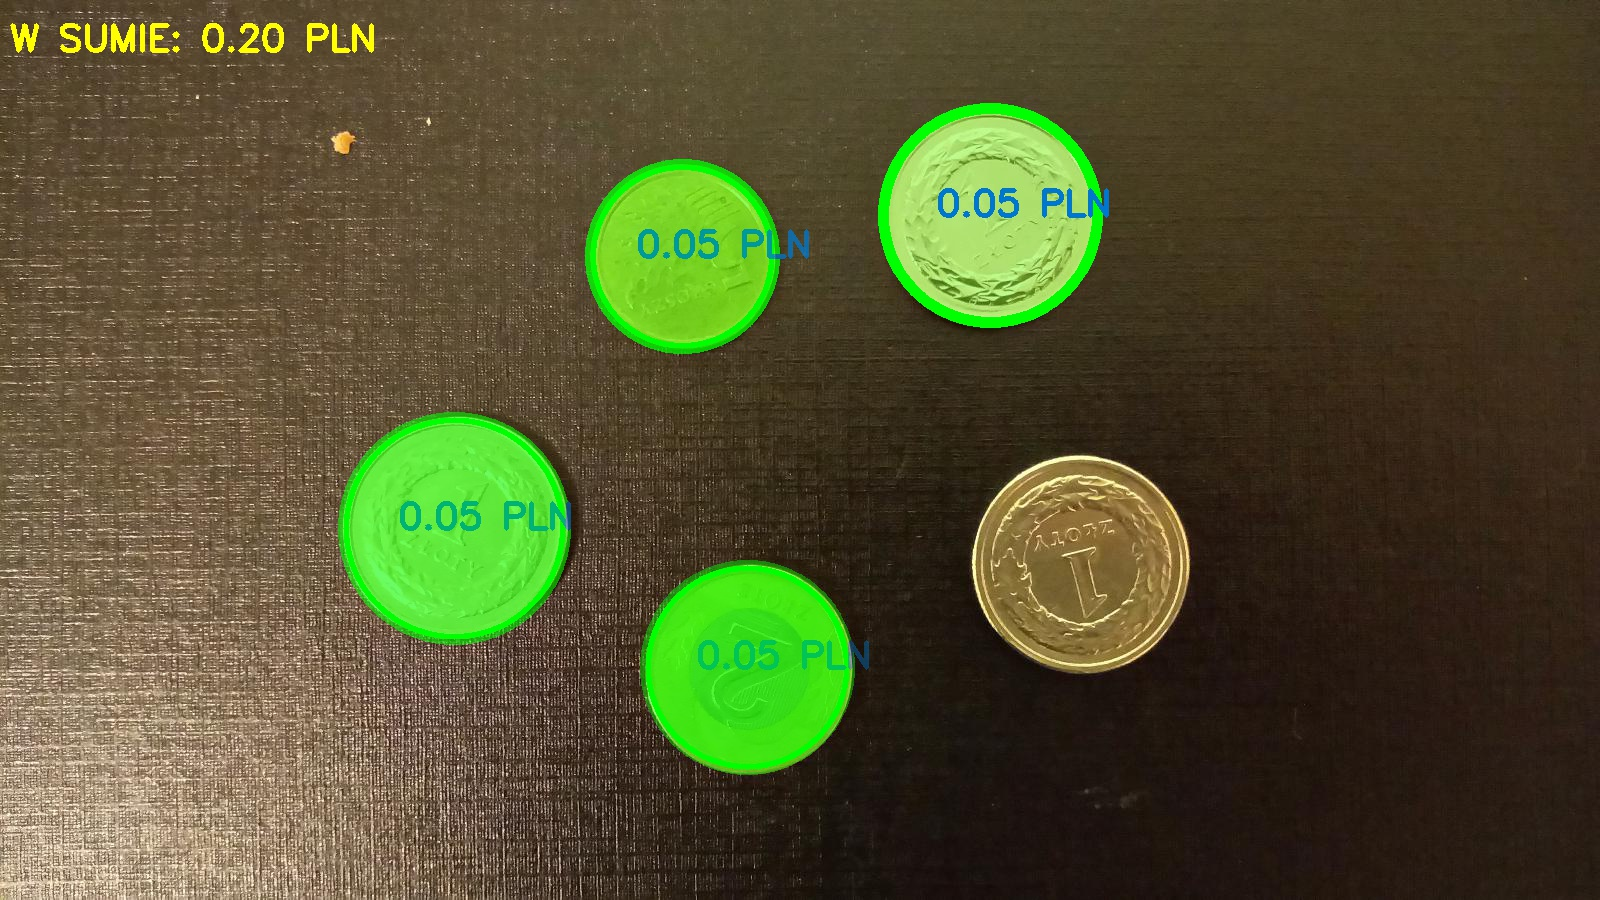
\includegraphics[width=0.4\textwidth]{bad_005.jpg}
        }
    \end{center}
    \caption{Błędnie rozpoznane obrazki}
   \label{fig:subfigures}
\end{figure}
\section{Bibliografia}

Przygotując projekt, bazowaliśmy na wiedzy dostępnej w Internecie. Szczególnie przydatne okazały się:

\begin{itemize}
    \item \href{https://docs.opencv.org/3.0-beta/index.html}{OpenCV documentation 3.0}
    \item \href{http://scikit-image.org/docs/dev/}{Skimage 0.14-dev documentation}
    \item \href{https://stackoverflow.com/}{Stack Overflow}
    \item \href{https://google.com/}{Uncle Google}
\end{itemize}

\end{document}
